\section{Ergebnisse}

\begin{figure}[t]
	\centering
	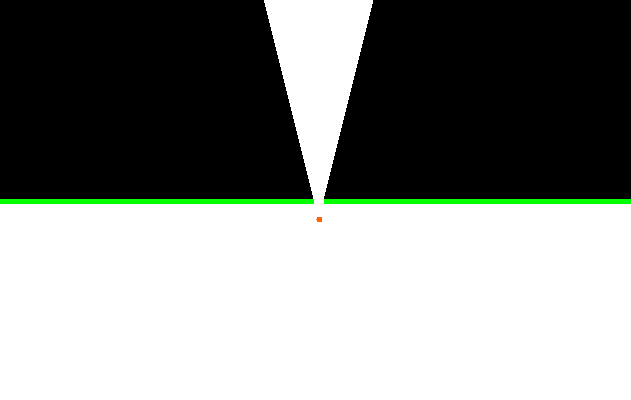
\includegraphics[width=\columnwidth]{images/ergebnis_3.png}
	\caption{Harter Schatten}
	\label{fig:ergeb4}
\end{figure}

Das Ziel der Berechnung von Schatten ist die Darstellung möglichst real wirkender Beleuchtung. In
der realen Welt werfen Lichter, wenn sie auf undurchsichtige Objekte treffen für gewöhnlich, keine
harten Schatten, wie in Abbildung \ref{fig:ergeb4}.

\begin{figure}[t]
	\centering
	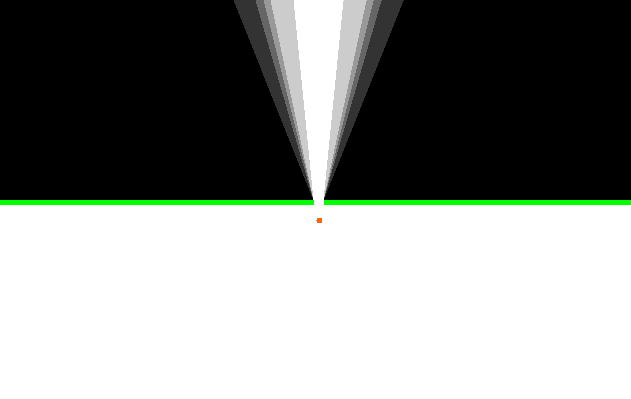
\includegraphics[width=\columnwidth]{images/ergebnis_2.png}
	\caption{Annäherung weicher Schatten}
	\label{fig:ergeb3}
\end{figure}

Weichere Schatten, wie in Abbildung \ref{fig:ergeb3}, können durch das Darstellen einer Lichtquelle
als Menge von leicht versetzten Lichtquellen erreicht werden.

\begin{figure}[t]
	\centering
	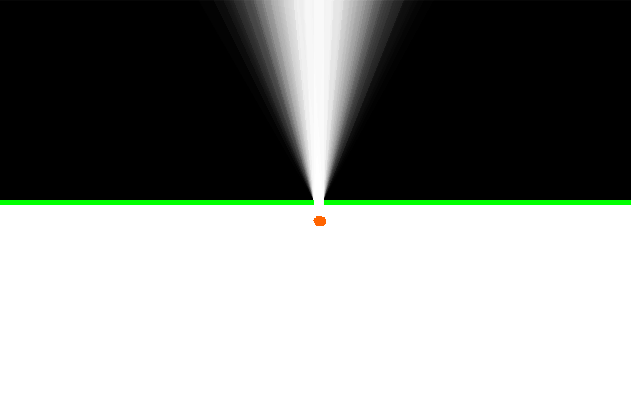
\includegraphics[width=\columnwidth]{images/ergebnis.png}
	\caption{Weiche Schatten}
	\label{fig:ergeb2}
\end{figure}

Durch eine weitere Erhöhung der Zahl, der Lichtquellen, kann eine noch realistischere Annäherung
vorgenommen werden. Umso mehr Lichtquellen bei der Annäherung verwendet werden, desto glatter ist
der Verlauf zwischen Schatten und Licht.

\begin{figure}[t]
	\centering
	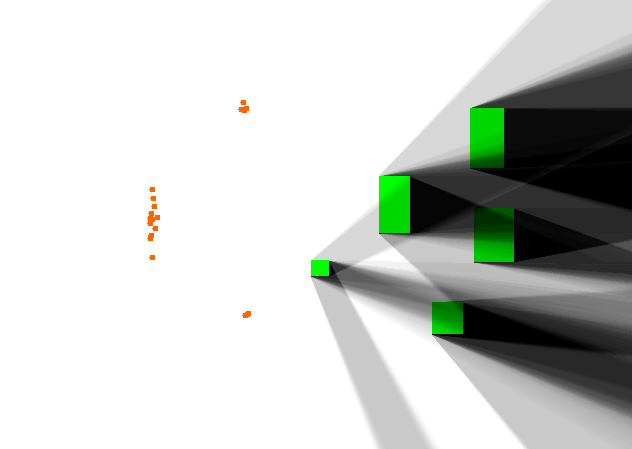
\includegraphics[width=\columnwidth]{images/ergebnis_4.png}
	\caption{Komplexe Szene}
	\label{fig:ergeb1}
\end{figure}

Abbildung \ref{fig:ergeb1} zeigt eine Szene mit vielen Lichtquellen und schattenwerfenden Objekten.
Zum einen wird hier ein weiteres Mal der an \ref{fig:ergeb2} gezeigte Effekt sichtbar. Schatten
sind nah am Objekt noch sehr hart und werden mit wachsendem Abstand zum schattenwerfenden Objekt
weicher. Zum anderen sieht man die Überlagerung von Schatten mehrerer Lichtquellen. Je nachdem wie
viele Lichtquellen auf ein Pixel scheinen, wird dieses mehr oder weniger hell eingefärbt. Durch die
Annäherung großer flächenartiger Lichtquellen durch viel kleine Punktlichter entstehen Umbra,
Penumbra und Antumbra.
